% Versuchsvorbereitende Aufgaben (Kapitel 2)
\section{Parallelschaltung von Transformatoren}\label{sec:a1}

\begin{aufgabe}{Aufgabenstellung}
Geben Sie einige Schaltgruppenkombinationen an, die parallelgeschaltet werden können. Was ist bei der Parallelschaltung von Transformatoren darüber hinaus zu beachten?
\end{aufgabe}

\textbf{Schaltgruppenkombinationen.} Zwei Transformatoren dürfen parallelgeschaltet werden, wenn sie dieselbe Kennzahl (Uhrzeigerzahl, $\varphi = \text{Kennzahl}\cdot\SI{30}{\degree}$) besitzen, da sonst zwischen den Sekundärseiten eine Spannungsdifferenz auftritt und ein Ausgleichsstrom fließt. Nach Abbildung~1.1 ergeben sich folgende Gruppen:

\begin{center}
\begin{tabular}{@{}cl@{}}
\toprule
Kennzahl & parallelschaltbare Schaltgruppen\\
\midrule
0  & Dd0 $\parallel$ Yy0 $\parallel$ Dz0\\
5  & Dy5 $\parallel$ Yd5 $\parallel$ Yz5\\
6  & Dd6 $\parallel$ Yy6 $\parallel$ Dz6\\
11 & Dy11 $\parallel$ Yd11 $\parallel$ Yz11\\
\bottomrule
\end{tabular}
\end{center}

Darüber hinaus lassen sich Transformatoren \emph{verschiedener} Kennzahl durch Vertauschen von Anschlüssen anpassen:
\begin{itemize}[nosep]
  \item Kennzahlen $0$, $4$, $8$ (sowie $2$, $6$, $10$) gehen durch \emph{zyklisches} Vertauschen der Außenleiter ineinander über (Drehung um $\pm\SI{120}{\degree}$).
  \item Kennzahlen $5$ und $11$ können durch Vertauschen zweier Außenleiter aneinander angepasst werden (z.\,B.\ Dy5 $\parallel$ Dy11).
\end{itemize}

\textbf{Weitere Bedingungen für die Parallelschaltung:}
\begin{itemize}[nosep]
  \item \textbf{Gleiche Nennspannungen bzw.\ gleiches Übersetzungsverhältnis} $\ue$ auf Ober- und Unterspannungsseite. Abweichungen führen zu Ausgleichsströmen (Kreisströmen) schon im Leerlauf.
  \item \textbf{Gleiche relative Kurzschlussspannung} $u_\mathrm{k}$ (zulässige Abweichung etwa $\SI{10}{\percent}$). Die Last teilt sich umgekehrt proportional zu $u_\mathrm{k}$ auf:
  \begin{equation*}
    \frac{S_1}{S_2} = \frac{S_\mathrm{N1}/u_\mathrm{k1}}{S_\mathrm{N2}/u_\mathrm{k2}}
  \end{equation*}
  Der Transformator mit dem kleineren $u_\mathrm{k}$ wird zuerst überlastet.
  \item \textbf{Ähnliches Verhältnis $R_\mathrm{k}/X_\mathrm{k}$} (gleicher Kurzschlusswinkel $\varphi_\mathrm{k}$), damit sich die Teilströme phasenrichtig addieren.
  \item \textbf{Nennleistungsverhältnis} nicht größer als etwa $3:1$.
  \item \textbf{Gleiche Frequenz und gleiche Phasenfolge (Drehsinn)}.
\end{itemize}

\section{Ströme, Spannungen und Scheinleistung}\label{sec:a2}

\begin{aufgabe}{Aufgabenstellung}
Bestimmen Sie für die Schaltungen in Abbildung~2.1 die maximal möglichen Ströme und Nennspannungen auf der Primär- und der Sekundärseite sowie die Trafo-Scheinleistung. Nehmen Sie hierfür die Daten des Trafos aus dem Laborversuch.
\end{aufgabe}

\textbf{Nenndaten des Prüflings (Tabelle~2):}
\begin{center}
\begin{tabular}{@{}lll@{}}
\toprule
Größe & Primär & Sekundär\\
\midrule
Nennspannung & $\SI{220}{V}$ je Strang & $\SI{110}{V}$ je Halbstrang\\
Nennstrom & $\SI{45.5}{A}$ je Strang & $\SI{45.5}{A}$ je Halbstrang\\
\bottomrule
\end{tabular}
\end{center}
Die Primärseite ist in allen Schaltungen in Stern geschaltet. Jeder Sekundärstrang besteht aus zwei Halbsträngen (je fünf Wicklungsteile in Reihe), die in Reihe oder parallel geschaltet werden können. Damit gilt für die Stranggrößen:
\begin{equation*}
  \text{Reihenschaltung: } \SI{220}{V},\ \SI{45.5}{A}
  \qquad
  \text{Parallelschaltung: } \SI{110}{V},\ \SI{91}{A}
\end{equation*}

\begin{hinweis}[Zuordnung der Schaltungen in Abbildung 2.1 der Versuchsanleitung]
Die vier Schaltungen werden im Folgenden so bezeichnet:\\
\textbf{(a)}~oben links: Sekundär Stern, beide Halbstränge je Strang in \emph{Reihe}.\quad
\textbf{(b)}~oben rechts: Sekundär Stern, beide Halbstränge je Strang \emph{parallel}.\\
\textbf{(c)}~unten links: Sekundär Stern, nur \emph{ein} Halbstrang je Strang.\quad
\textbf{(d)}~unten rechts: Sekundär \emph{Zickzack} aus Halbsträngen verschiedener Schenkel.
\end{hinweis}

\paragraph{Rechenweg}

\textbf{Primärseite (Stern):}
\begin{equation*}
  U_{1,\mathrm{Str}} = \SI{220}{V}, \qquad
  U_{1} = \sqrt{3}\cdot\SI{220}{V} \approx \SI{381}{V}, \qquad
  I_{1,\max} = \SI{45.5}{A}
\end{equation*}

\textbf{(a) Y/Y, Halbstränge in Reihe:}
\begin{align*}
  U_{2,\mathrm{Str}} &= 2\cdot\SI{110}{V} = \SI{220}{V}, &
  U_2 &= \sqrt{3}\cdot\SI{220}{V} \approx \SI{381}{V}, &
  I_2 &= \SI{45.5}{A}\\
  \ue &= \frac{U_1}{U_2} = 1, &
  I_1 &= \SI{45.5}{A}, &
  S &= \sqrt{3}\cdot\SI{381}{V}\cdot\SI{45.5}{A} \approx \SI{30}{kVA}
\end{align*}

\textbf{(b) Y/Y, Halbstränge parallel:}
\begin{align*}
  U_{2,\mathrm{Str}} &= \SI{110}{V}, &
  U_2 &= \sqrt{3}\cdot\SI{110}{V} \approx \SI{190.5}{V}, &
  I_2 &= 2\cdot\SI{45.5}{A} = \SI{91}{A}\\
  \ue &= \frac{\SI{381}{V}}{\SI{190.5}{V}} = 2, &
  I_1 &= \frac{I_2}{\ue} = \SI{45.5}{A}, &
  S &= \sqrt{3}\cdot\SI{190.5}{V}\cdot\SI{91}{A} \approx \SI{30}{kVA}
\end{align*}

\textbf{(c) Y/Y, ein Halbstrang je Strang:}
\begin{align*}
  U_{2,\mathrm{Str}} &= \SI{110}{V}, &
  U_2 &= \SI{190.5}{V}, &
  I_2 &= \SI{45.5}{A}\\
  \ue &= 2, &
  I_1 &= \frac{I_2}{\ue} = \SI{22.75}{A}, &
  S &= \sqrt{3}\cdot\SI{190.5}{V}\cdot\SI{45.5}{A} \approx \SI{15}{kVA}
\end{align*}
Der Sekundärstrom ist durch den Halbstrang begrenzt, daher wird die Primärseite nur zur Hälfte ausgelastet.

\textbf{(d) Y/Zickzack:} Jede Zickzack-Phase besteht aus zwei Halbsträngen verschiedener Schenkel (Spannungen um $\SI{120}{\degree}$ verschoben), die geometrisch addiert werden:
\begin{align*}
  U_{2,\mathrm{Str}} &= |\underline{U}_\mathrm{U} - \underline{U}_\mathrm{V}| = \sqrt{3}\cdot\SI{110}{V} \approx \SI{190.5}{V}, &
  U_2 &= \sqrt{3}\cdot U_{2,\mathrm{Str}} = 3\cdot\SI{110}{V} = \SI{330}{V}\\
  I_2 &= \SI{45.5}{A}, &
  \ue &= \frac{\SI{381}{V}}{\SI{330}{V}} = \frac{2}{\sqrt{3}} \approx 1{,}155\\
  I_1 &= \frac{I_2}{\ue} \approx \SI{39.4}{A}, &
  S &= \sqrt{3}\cdot\SI{330}{V}\cdot\SI{45.5}{A} \approx \SI{26}{kVA}
\end{align*}
Die Scheinleistung beträgt nur $\frac{\sqrt{3}}{2} \approx \SI{86.6}{\percent}$ der Nennleistung, da sich die Halbstrangspannungen geometrisch statt arithmetisch addieren. Sekundärseitig fließt ein höherer Strom als primärseitig.

\begin{ergebnis}[Ergebnis Aufgabe 2]
\centering
\small
\setlength{\tabcolsep}{4pt}
\begin{tabular}{@{}cl*{7}{r}@{}}
\toprule
 & Sek.-Schaltung & $U_1$ & $I_1$ & $U_{2,\mathrm{Str}}$ & $U_2$ & $I_2$ & $\ue$ & $S$\\
 &  & in V & in A & in V & in V & in A & & in kVA\\
\midrule
(a) & Y, Reihe    & 381 & 45,5  & 220   & 381   & 45,5 & 1     & 30\\
(b) & Y, parallel & 381 & 45,5  & 110   & 190,5 & 91   & 2     & 30\\
(c) & Y, 1 Halbstr. & 381 & 22,75 & 110 & 190,5 & 45,5 & 2     & 15\\
(d) & Zickzack    & 381 & 39,4  & 190,5 & 330   & 45,5 & 1,155 & 26\\
\bottomrule
\end{tabular}
\end{ergebnis}

\section{Klemmenbezeichnungen und Schaltgruppen}\label{sec:a3}

\begin{aufgabe}{Aufgabenstellung}
Ergänzen Sie die Klemmenbezeichnungen in Abbildung~2.1. Welche Phasenverschiebungen zwischen Primär- und Sekundärseite sind bei unveränderter Schaltung der Primärwicklung für die obigen Beispiele möglich? Schaltgruppe und Gradzahl. Orientieren Sie sich bei der Klemmenbezeichnung am Prüfling in Abbildung~3.2.
\end{aufgabe}

\textbf{Primärseite (alle Schaltungen):} Die beiden Wicklungsteile je Strang sind in Reihe geschaltet (U4--U3). Die Netzanschlüsse sind U1, V1, W1 (oben), der Sternpunkt wird aus U2, V2, W2 (unten) gebildet.

\textbf{Sekundärseite:} Je Schenkel gibt es zwei Halbstränge, z.\,B.\ für Schenkel U die Halbstränge 2U1--2U2 und 3U1--3U2 (entsprechend V und W). Die fünf Wicklungsteile eines Halbstrangs sind bereits verbunden.

\begin{center}
\small
\renewcommand{\arraystretch}{1.25}
\begin{tabular}{@{}cp{4.3cm}p{4.3cm}p{2.6cm}@{}}
\toprule
 & Sternpunkt / Brücken & Ausgangsklemmen & Schaltgruppe\\
\midrule
(a) & Brücken 2U2--3U1, 2V2--3V1, 2W2--3W1; Sternpunkt: 2U1, 2V1, 2W1 & 3U2, 3V2, 3W2 & Yy6 (180°)\\
    & Anschlüsse vertauscht: Sternpunkt 3U2, 3V2, 3W2 & 2U1, 2V1, 2W1 & Yy0 (0°)\\
\midrule
(b) & Parallelschaltung 2U1$\parallel$3U1 usw.; Sternpunkt: 2U1, 3U1, 2V1, 3V1, 2W1, 3W1 & 2U2$\parallel$3U2, 2V2$\parallel$3V2, 2W2$\parallel$3W2 & Yy6 (180°)\\
    & Anschlüsse vertauscht & 2U1$\parallel$3U1, \ldots & Yy0 (0°)\\
\midrule
(c) & Sternpunkt: 2U1, 2V1, 2W1 & 2U2, 2V2, 2W2 & Yy6 (180°)\\
    & Anschlüsse vertauscht: Sternpunkt 2U2, 2V2, 2W2 & 2U1, 2V1, 2W1 & Yy0 (0°)\\
\bottomrule
\end{tabular}
\end{center}

Bei Schaltungen (a) bis (c) liegen Primär- und Sekundärwicklung auf demselben Schenkel. Die Sekundärspannung ist daher entweder in Phase oder genau gegenphasig zur Primärspannung. Je nachdem, ob Wicklungsanfang oder Wicklungsende als Klemme genutzt wird, ergeben sich:
\begin{equation*}
  \text{Yy0: } 0\cdot\SI{30}{\degree} = \SI{0}{\degree}
  \qquad\text{oder}\qquad
  \text{Yy6: } 6\cdot\SI{30}{\degree} = \SI{180}{\degree}
\end{equation*}

\textbf{(d) Zickzack:} Hier werden Halbstränge \emph{verschiedener} Schenkel in Reihe geschaltet. Die Phasenspannung ist die Differenz zweier um $\SI{120}{\degree}$ verschobener Strangspannungen.

\begin{center}
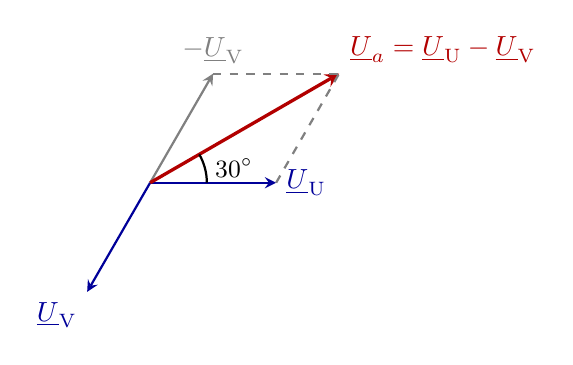
\begin{tikzpicture}[scale=0.8,>=stealth,thick]
  \draw[->,blue!60!black] (0,0) -- (2,0) node[right] {$\underline{U}_\mathrm{U}$};
  \draw[->,blue!60!black] (0,0) -- (-1,-1.732) node[below left] {$\underline{U}_\mathrm{V}$};
  \draw[->,gray] (0,0) -- (1,1.732) node[above] {$-\underline{U}_\mathrm{V}$};
  \draw[->,red!70!black,very thick] (0,0) -- (3,1.732) node[above right] {$\underline{U}_a=\underline{U}_\mathrm{U}-\underline{U}_\mathrm{V}$};
  \draw[dashed,gray] (2,0) -- (3,1.732);
  \draw[dashed,gray] (1,1.732) -- (3,1.732);
  \draw (0.9,0) arc (0:30:0.9) node[midway,right] {\small $30^\circ$};
\end{tikzpicture}
\end{center}

\begin{equation*}
  |\underline{U}_a| = \sqrt{3}\,U_\mathrm{Str}\ \text{(Halbstrang)}, \qquad
  \text{Lage: } \pm\SI{30}{\degree}\ \text{bzw.}\ \SI{180}{\degree}\pm\SI{30}{\degree}
\end{equation*}

Je nach Wahl der beteiligten Halbstränge und ihrer Polung sind bei gleicher Primärschaltung vier Schaltgruppen möglich:

\begin{center}
\begin{tabular}{@{}llcl@{}}
\toprule
Schaltgruppe & Verschaltung der Phase $a$ & Lage von $\underline{U}_a$ (voreilend) & Phasenverschiebung\\
\midrule
Yz11 & $\underline{U}_\mathrm{U}-\underline{U}_\mathrm{V}$ & $+\SI{30}{\degree}$  & $11\cdot\SI{30}{\degree}=\SI{330}{\degree}$\\
Yz5  & $\underline{U}_\mathrm{V}-\underline{U}_\mathrm{U}$ & $+\SI{210}{\degree}$ & $5\cdot\SI{30}{\degree}=\SI{150}{\degree}$\\
Yz1  & $\underline{U}_\mathrm{U}-\underline{U}_\mathrm{W}$ & $-\SI{30}{\degree}$  & $1\cdot\SI{30}{\degree}=\SI{30}{\degree}$\\
Yz7  & $\underline{U}_\mathrm{W}-\underline{U}_\mathrm{U}$ & $+\SI{150}{\degree}$ & $7\cdot\SI{30}{\degree}=\SI{210}{\degree}$\\
\bottomrule
\end{tabular}
\end{center}

\textbf{Klemmenbezeichnung für Yz11} (Phase $a$ aus Halbstrang 2U vorwärts und 3V rückwärts, entsprechend zyklisch weiter):
\begin{center}
\small
\begin{tabular}{@{}lccc@{}}
\toprule
 & Klemme & Brücke & Sternpunkt\\
\midrule
Phase 1 & 2U1 & 2U2--3V2 & 3V1\\
Phase 2 & 2V1 & 2V2--3W2 & 3W1\\
Phase 3 & 2W1 & 2W2--3U2 & 3U1\\
\bottomrule
\end{tabular}
\end{center}
Die Sternpunktklemmen 3U1, 3V1 und 3W1 werden miteinander verbunden. Für \textbf{Yz5} wird jede Phase in umgekehrter Richtung durchlaufen: Klemme 2U2, Brücke 2U1--3V1, Sternpunkt 3V2 (entsprechend für V und W).

\begin{ergebnis}[Ergebnis Aufgabe 3]
\begin{itemize}[nosep]
  \item Schaltungen (a), (b), (c) (Yy): \textbf{Yy0 ($\SI{0}{\degree}$)} und \textbf{Yy6 ($\SI{180}{\degree}$)}.
  \item Schaltung (d) (Yz): \textbf{Yz1 ($\SI{30}{\degree}$)}, \textbf{Yz5 ($\SI{150}{\degree}$)}, \textbf{Yz7 ($\SI{210}{\degree}$)}, \textbf{Yz11 ($\SI{330}{\degree}$)}.
\end{itemize}
\end{ergebnis}

\section{Rush-Effekt}\label{sec:a4}

\begin{aufgabe}{Aufgabenstellung}
Was ist der Rush-Effekt bei Transformatoren und wodurch wird dieser ausgelöst? Beschreiben Sie mehrere Maßnahmen, um den Rush-Effekt zu reduzieren.
\end{aufgabe}

\textbf{Was ist der Rush-Effekt?} Beim Einschalten eines Transformators (meist im Leerlauf) tritt kurzzeitig ein sehr hoher Einschaltstromstoß (Inrush-Strom) auf. Er kann ein Vielfaches des Nennstroms erreichen (typisch das $5$- bis $10$-fache, im Extremfall mehr) und klingt erst nach mehreren Perioden bis Sekunden ab. Der Strom ist stark unsymmetrisch (Gleichanteil) und reich an Oberschwingungen, besonders der 2.~Harmonischen.

\textbf{Ursache:} Der magnetische Fluss kann sich nicht sprunghaft ändern. Wird die Spannung $u(t)=\hat{u}\sin(\omega t+\alpha)$ zum Zeitpunkt $t=0$ aufgeschaltet, gilt für den Fluss
\begin{equation*}
  \Phi(t) = \underbrace{-\hat{\Phi}\cos(\omega t+\alpha)}_{\text{stationär}}
            + \underbrace{\hat{\Phi}\cos\alpha}_{\text{Gleichanteil}}
            + \Phi_\mathrm{R},
  \qquad \hat{\Phi}=\frac{\hat{u}}{\omega N}
\end{equation*}
mit der Remanenz $\Phi_\mathrm{R}$ des Kerns. Im ungünstigsten Fall (Einschalten im Spannungsnulldurchgang, $\alpha=0$, Remanenz gleichgerichtet) erreicht der Fluss
\begin{equation*}
  \Phi_{\max} \approx 2\hat{\Phi} + \Phi_\mathrm{R}.
\end{equation*}
Da der Transformator im Nennbetrieb schon nahe an der Sättigungsgrenze arbeitet, geht der Kern in die Sättigung. Die Induktivität sinkt dort auf den Wert der Luftspule, und der Magnetisierungsstrom steigt stark nichtlinear an. Beim Einschalten im Spannungsmaximum ($\alpha=\SI{90}{\degree}$) tritt dagegen kein Gleichanteil auf und kein Rush-Effekt (bei $\Phi_\mathrm{R}=0$).

Der Einschaltstrom hängt damit ab von:
\begin{itemize}[nosep]
  \item dem Einschaltzeitpunkt (Schaltwinkel $\alpha$),
  \item der Remanenz des Kerns,
  \item der Sättigungskennlinie bzw.\ der Induktion im Nennbetrieb,
  \item der Netz- und Wicklungsimpedanz (bestimmt die Abklingzeit des Gleichanteils).
\end{itemize}

\textbf{Maßnahmen zur Reduzierung:}
\begin{itemize}[nosep]
  \item \textbf{Synchronisiertes Einschalten} (Point-on-Wave, z.\,B.\ mit Halbleiterrelais): Einschalten im Spannungsmaximum, bei Kenntnis der Remanenz mit angepasstem Winkel.
  \item \textbf{Vorwiderstände bzw.\ Einschaltstrombegrenzer} (z.\,B.\ Widerstand mit Überbrückungsschütz nach dem Hochlauf, NTC-Widerstände).
  \item \textbf{Spannung langsam hochfahren}: Stelltransformator oder Sanftanlauf (Phasenanschnitt, Softstarter), damit sich der Fluss stetig aufbaut.
  \item \textbf{Niedrigere Auslegungsinduktion} (größerer Eisenquerschnitt, mehr Abstand zur Sättigung) oder Luftspalt im Kern, wodurch die Remanenz sinkt. Nachteil: höhere Kosten, größeres Gewicht bzw.\ höherer Magnetisierungsstrom.
  \item \textbf{Entmagnetisieren} bzw.\ definierte Remanenz einstellen.
  \item \textbf{Sequentielles Einschalten} der Phasen bzw.\ mehrerer Transformatoren, damit sich die Einschaltströme nicht überlagern.
  \item \textbf{Netzimpedanz bzw.\ Vorschaltdrossel}: Eine größere Impedanz verringert die Stromspitze und beschleunigt das Abklingen.
\end{itemize}


%==================================================
